\chapter{Diagrams}

\section{Internet Content Languages}

\begin{figure}[H]
	\centering
	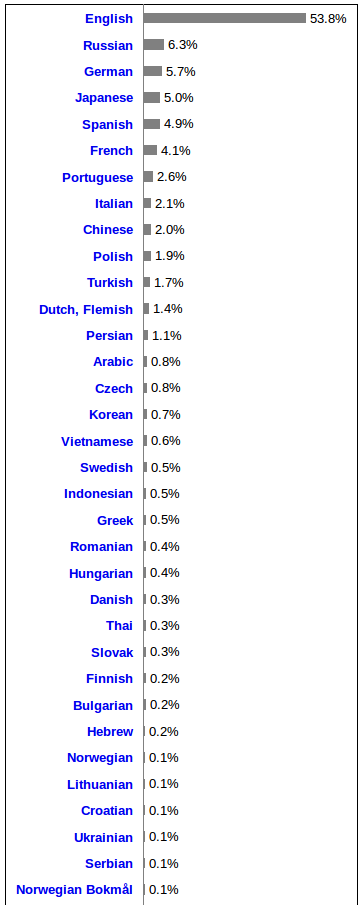
\includegraphics[height=30em]{diagrams/w3techsInternetContentLang.png}
	\caption[a figure]{\textit{Usage of content languages for websites [Screenshot]}. Retrieved from \url{http://w3techs.com/technologies/overview/content_language/all} (Online; accessed 19-February-2016)}
	\label{fig:w3techLang}
\end{figure}

\section{List of languages by number of native speakers}
\begin{figure}[H]
	\centering
	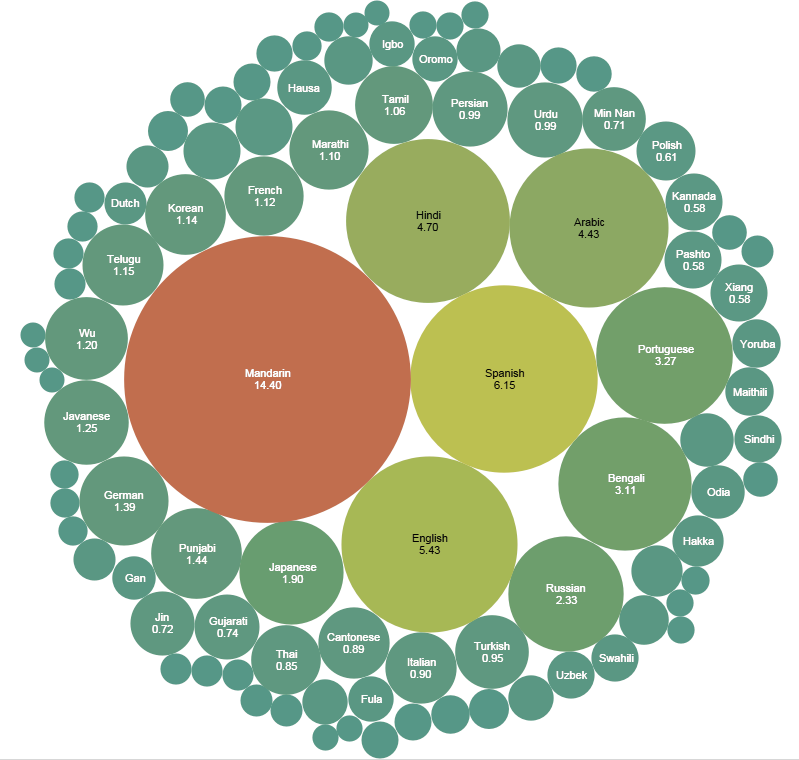
\includegraphics[width=\textwidth]{diagrams/List_of_languages_by_number_of_native_speakers.png}
	\caption[a figure]{Jroehl (2015). \textit{List of languages by number of native speakers, Packed bubbles.}. Retrieved from \url{https://en.wikipedia.org/wiki/List\_of\_languages\_by\_number\_of\_native\_speakers\#/media/File:List\_of\_languages\_by\_number\_of\_native\_speakers.png} (Online; accessed 19-February-2016)}
	\label{fig:listLang}
\end{figure}

\section{Lists of Wikipedias with over 1.000.000 articles}
\begin{figure}[H]
	\centering
	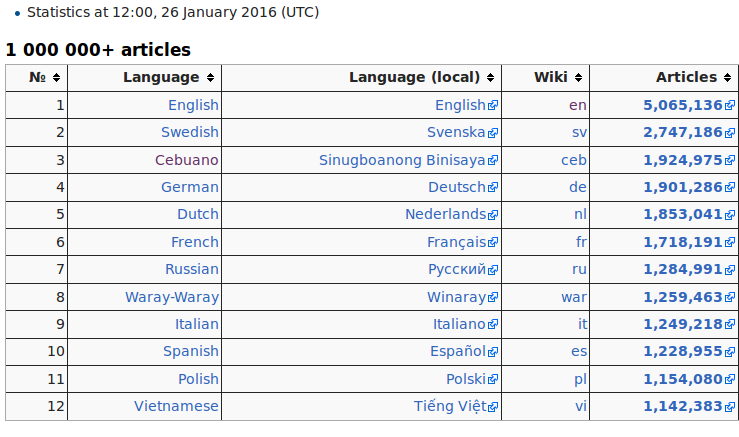
\includegraphics[width=\textwidth]{diagrams/list-of-wikis-articles.png}
	\caption[a figure]{\textit{List of Wikipedias with over 1.000.000 articles [Screenshot]}. Retrieved from \url{https://meta.wikimedia.org/wiki/List\_of\_Wikipedias} (Online; accessed 19-February-2016)}
	\label{fig:wikipedias-articles}
\end{figure}